\chapter{Anexo A}
\label{cap:AnexoA}

Este anexo se ha dedicado a varias figuras relevantes para el desarrollo de este documento, que se han ido mencionando a lo largo de su cuerpo.


\section{Diagramas de secuencia}
\label{ana:diagramassecuencia}
A continuación se muestran los diagramas de secuencia de los casos de uso más interesantes.

\begin{itemize}
	\item\textbf{Iniciar sesión}, en la figura \ref{Fig:dia_iniciarsesion}. También se muestra aquí, de manera opcional, cómo modificar la apariencia visual del programa.
	\item\textbf{Visualizar las notas del alumno}, en la figura \ref{Fig:dia_mainwindow} para las notas finales y en la figura \ref{Fig:dia_informealumno} para el informe general del alumno.
	\item\textbf{Crear una nueva prueba}, en la figura \ref{Fig:dia_nuevaprueba}.
	\item\textbf{Calificar una prueba}, en la figura \ref{Fig:dia_calificarprueba}.
	\item\textbf{Modificar una prueba}, en la figura \ref{Fig:dia_modificarprueba}.
	\item\textbf{Borrar una prueba}, en la figura \ref{Fig:dia_borrarprueba}.
	\item\textbf{Editar datos del usuario}, en la figura \ref{Fig:dia_editarusuario}.
	\item\textbf{Cargar alumnos}, en las figuras \ref{Fig:dia_cargaralumno} para un solo alumno y \ref{Fig:dia_cargaralumnos} para varios alumnos.
\end{itemize}.

\newpage

\begin{figure}[H]
\centering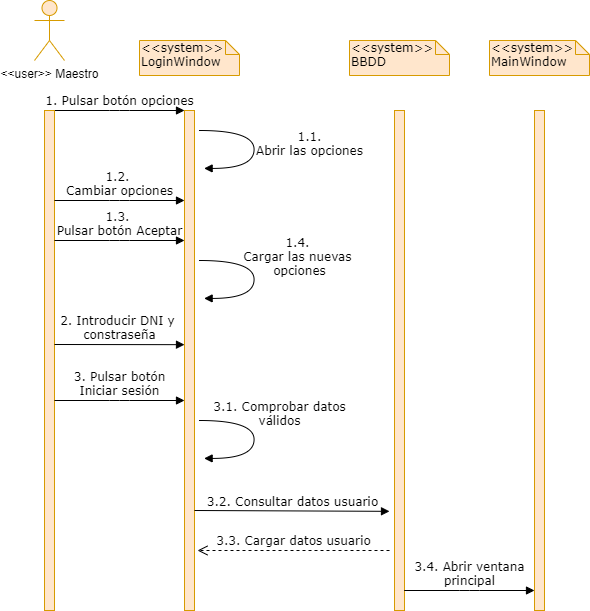
\includegraphics[width=0.75\linewidth]{figs/dia_iniciarsesion.png}
\caption{Diagrama de secuencia del inicio de sesión.}
\label{Fig:dia_iniciarsesion}
\end{figure}

\begin{figure}[H]
\centering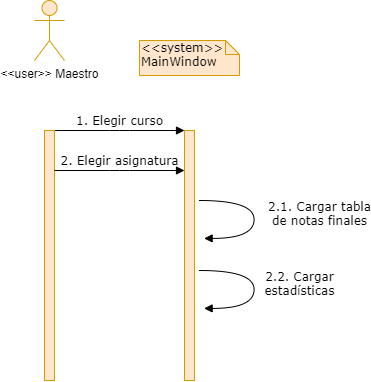
\includegraphics[width=0.5\linewidth]{figs/dia_mainwindow.png}
\caption{Diagrama de secuencia de la visualización de notas finales.}
\label{Fig:dia_mainwindow}
\end{figure}

\begin{figure}[H]
\centering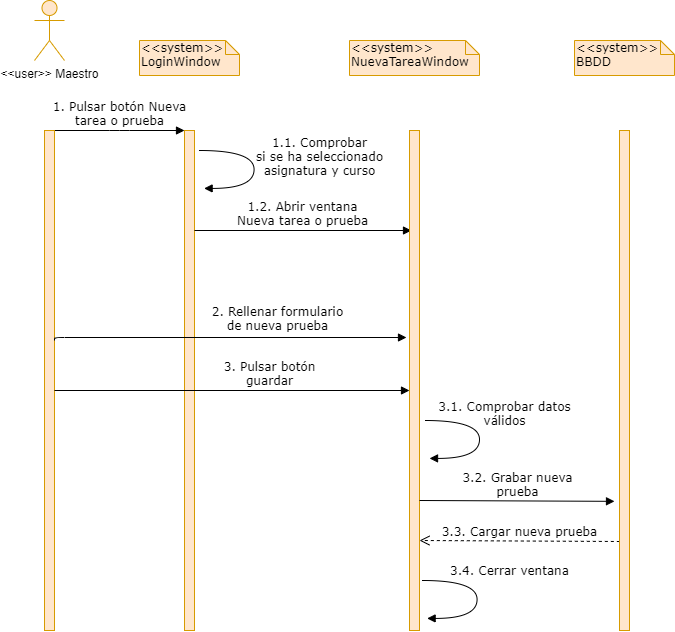
\includegraphics[width=0.75\linewidth]{figs/dia_nuevaprueba.png}
\caption{Diagrama de secuencia de la creación de una prueba nueva.}
\label{Fig:dia_nuevaprueba}
\end{figure}

\begin{figure}[H]
\centering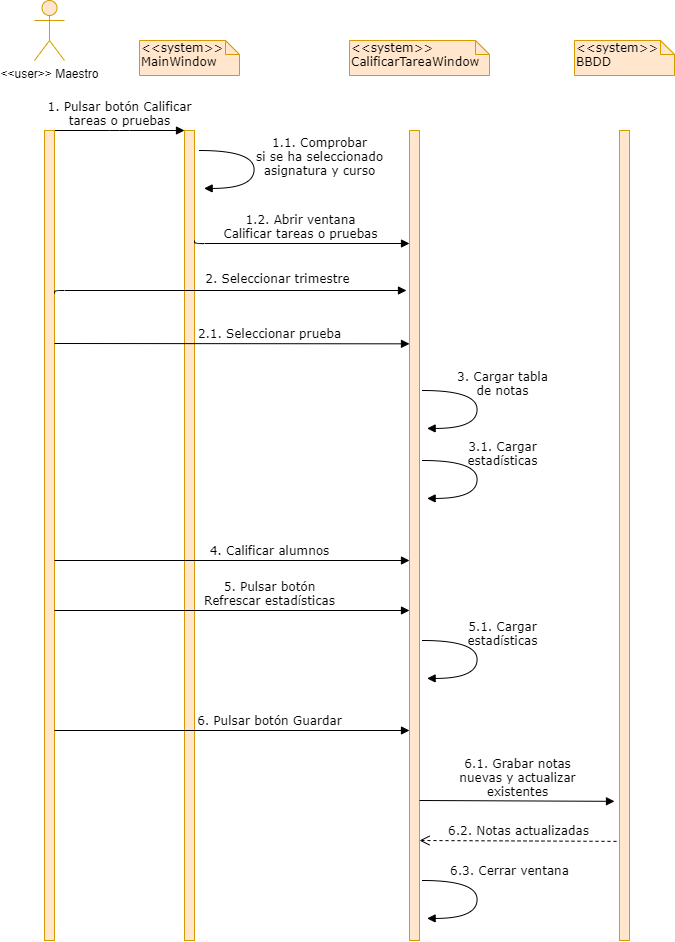
\includegraphics[width=1\linewidth]{figs/dia_calificarprueba.png}
\caption{Diagrama de secuencia de la calificación de una prueba.}
\label{Fig:dia_calificarprueba}
\end{figure}

\begin{figure}[H]
\centering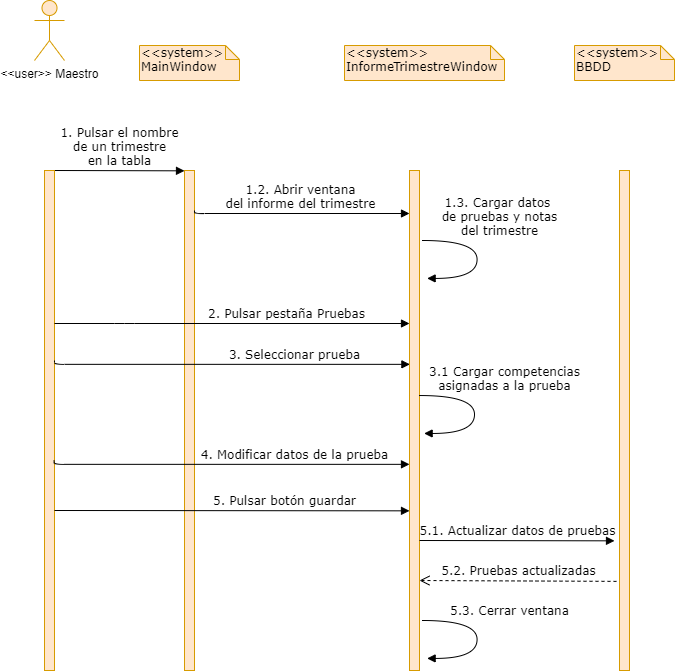
\includegraphics[width=1\linewidth]{figs/dia_modificarprueba.png}
\caption{Diagrama de secuencia de la modificación de una prueba.}
\label{Fig:dia_modificarprueba}
\end{figure}

\begin{figure}[H]
\centering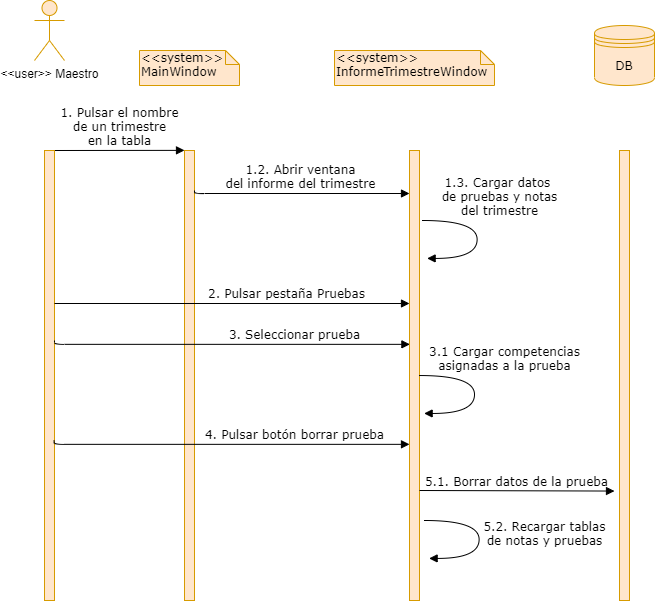
\includegraphics[width=0.75\linewidth]{figs/dia_borrarprueba.png}
\caption{Diagrama de secuencia del borrado de una prueba.}
\label{Fig:dia_borrarprueba}
\end{figure}

\begin{figure}[H]
\centering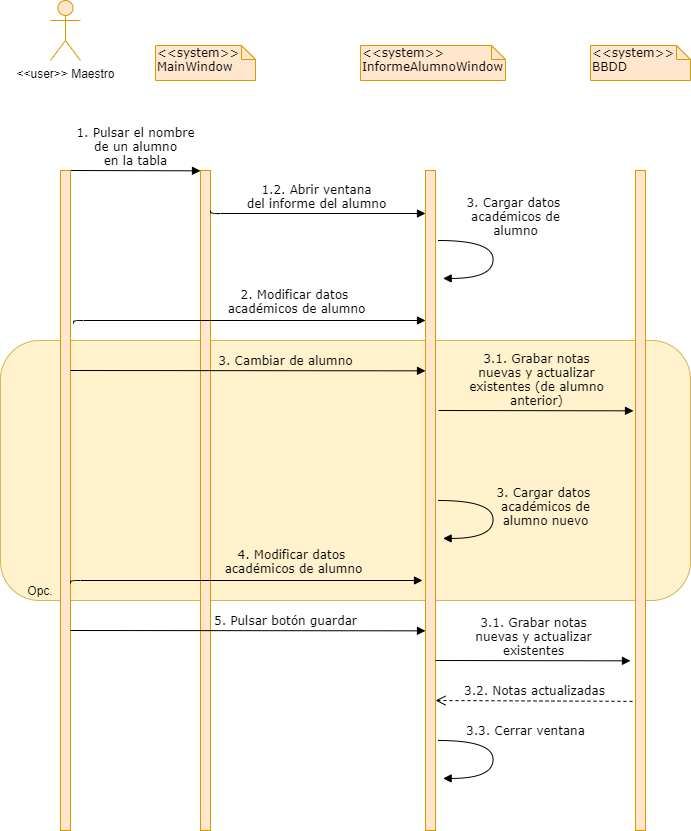
\includegraphics[width=1\linewidth]{figs/dia_informealumno.png}
\caption{Diagrama de secuencia de la visualización de todas las notas del alumno.}
\label{Fig:dia_informealumno}
\end{figure}

\begin{figure}[h]
\centering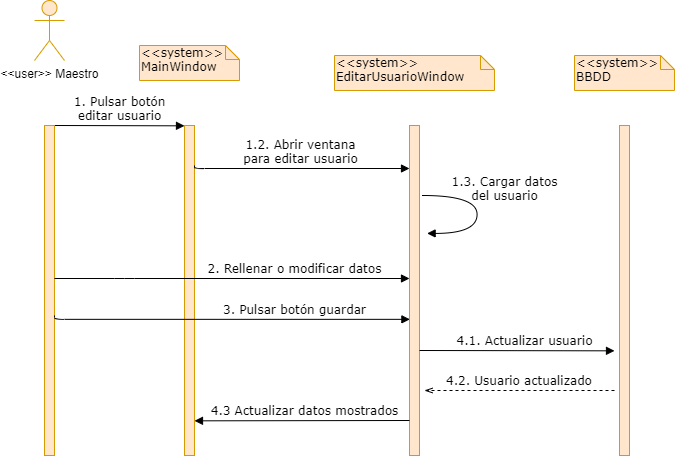
\includegraphics[width=0.75\linewidth]{figs/dia_editarusuario.png}
\caption{Diagrama de secuencia de la edición de los datos del usuario.}
\label{Fig:dia_editarusuario}
\end{figure}

\begin{figure}[H]
\centering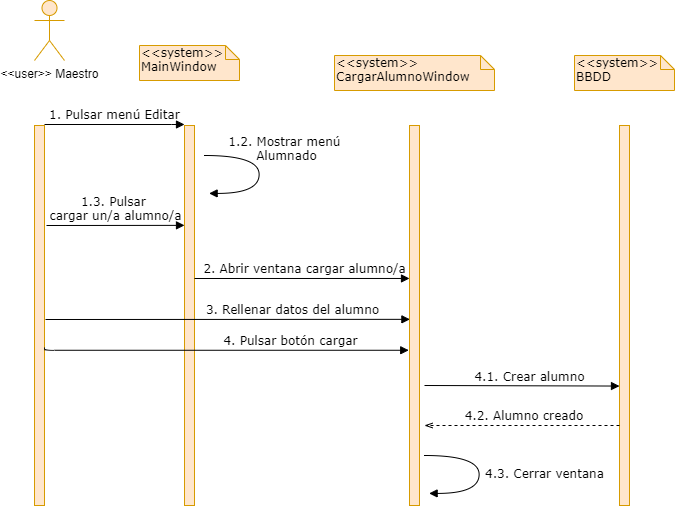
\includegraphics[width=0.75\linewidth]{figs/dia_cargaralumno.png}
\caption{Diagrama de secuencia de la carga de un alumno.}
\label{Fig:dia_cargaralumno}
\end{figure}

\begin{figure}[H]
\centering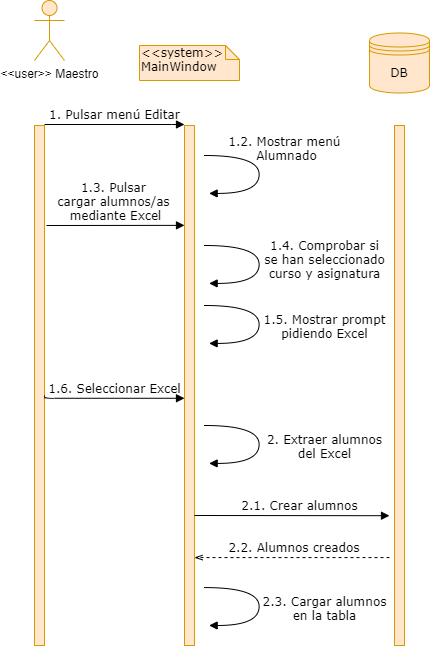
\includegraphics[width=0.5\linewidth]{figs/dia_cargaralumnos.png}
\caption{Diagrama de secuencia de la carga de varios alumnos.}
\label{Fig:dia_cargaralumnos}
\end{figure}

\section{Bocetos de la aplicación}
\label{ana:bocetos}
\begin{figure}[H]
\centering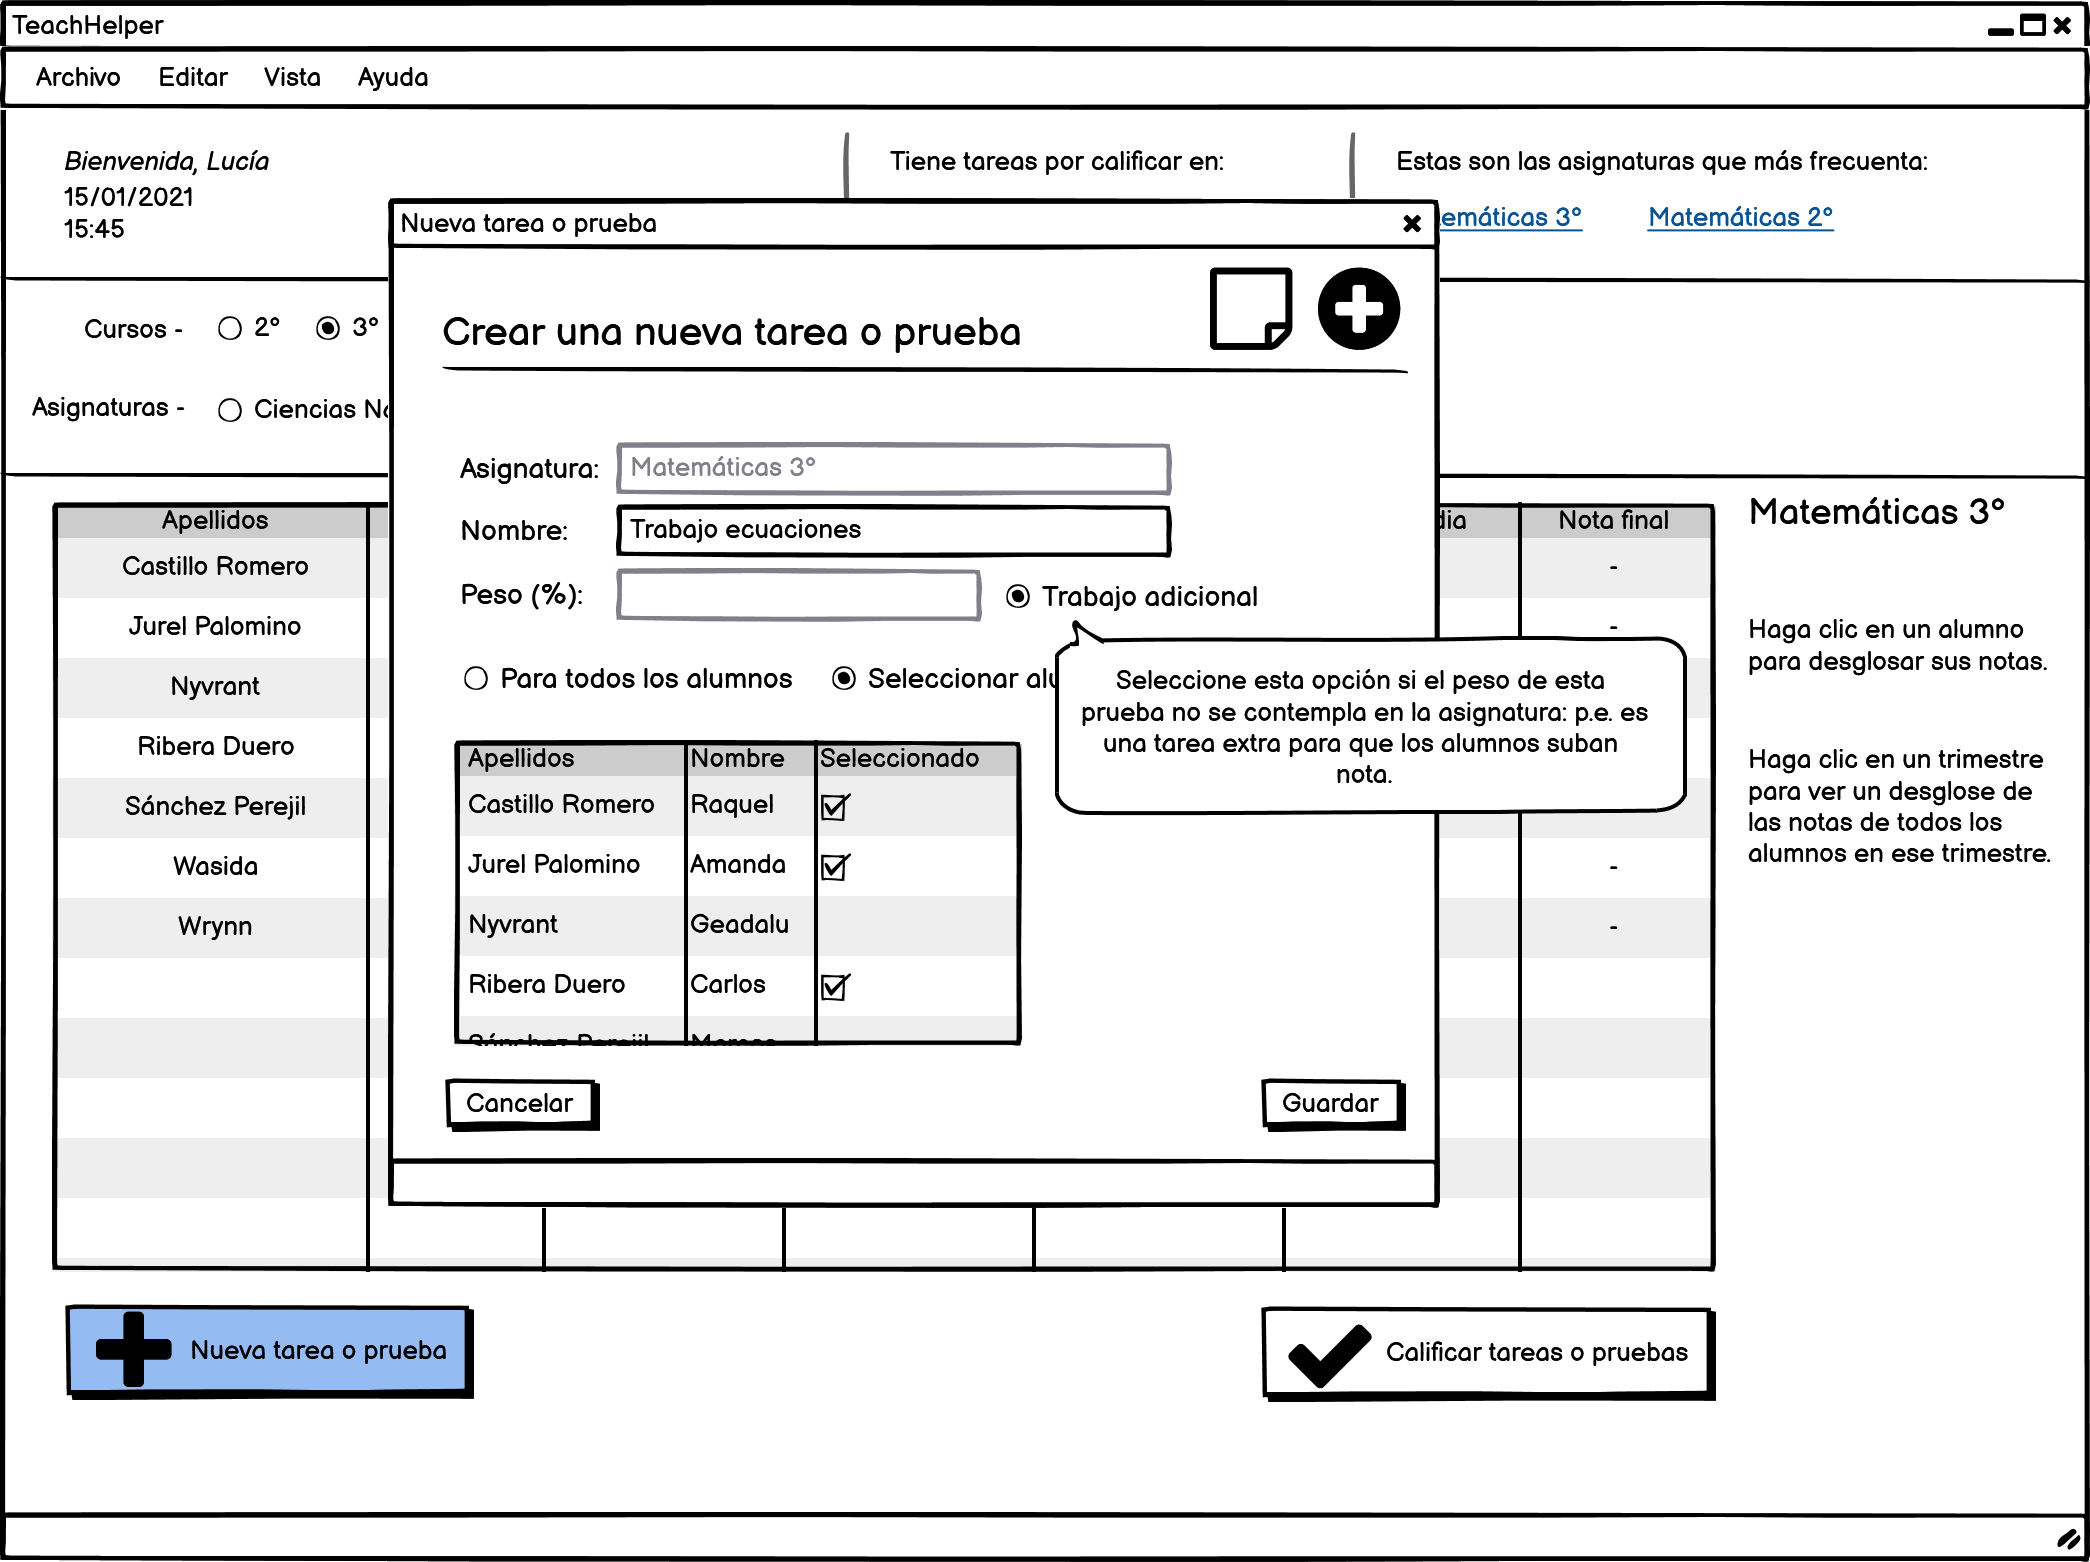
\includegraphics[width=1\linewidth]{figs/mockup_nuevatarea.png}
\caption{Prototipo de la creación de nuevas tareas o pruebas.}
\label{Fig:mockup_nuevatarea}
\end{figure}

\newpage

\begin{figure}[H]
\centering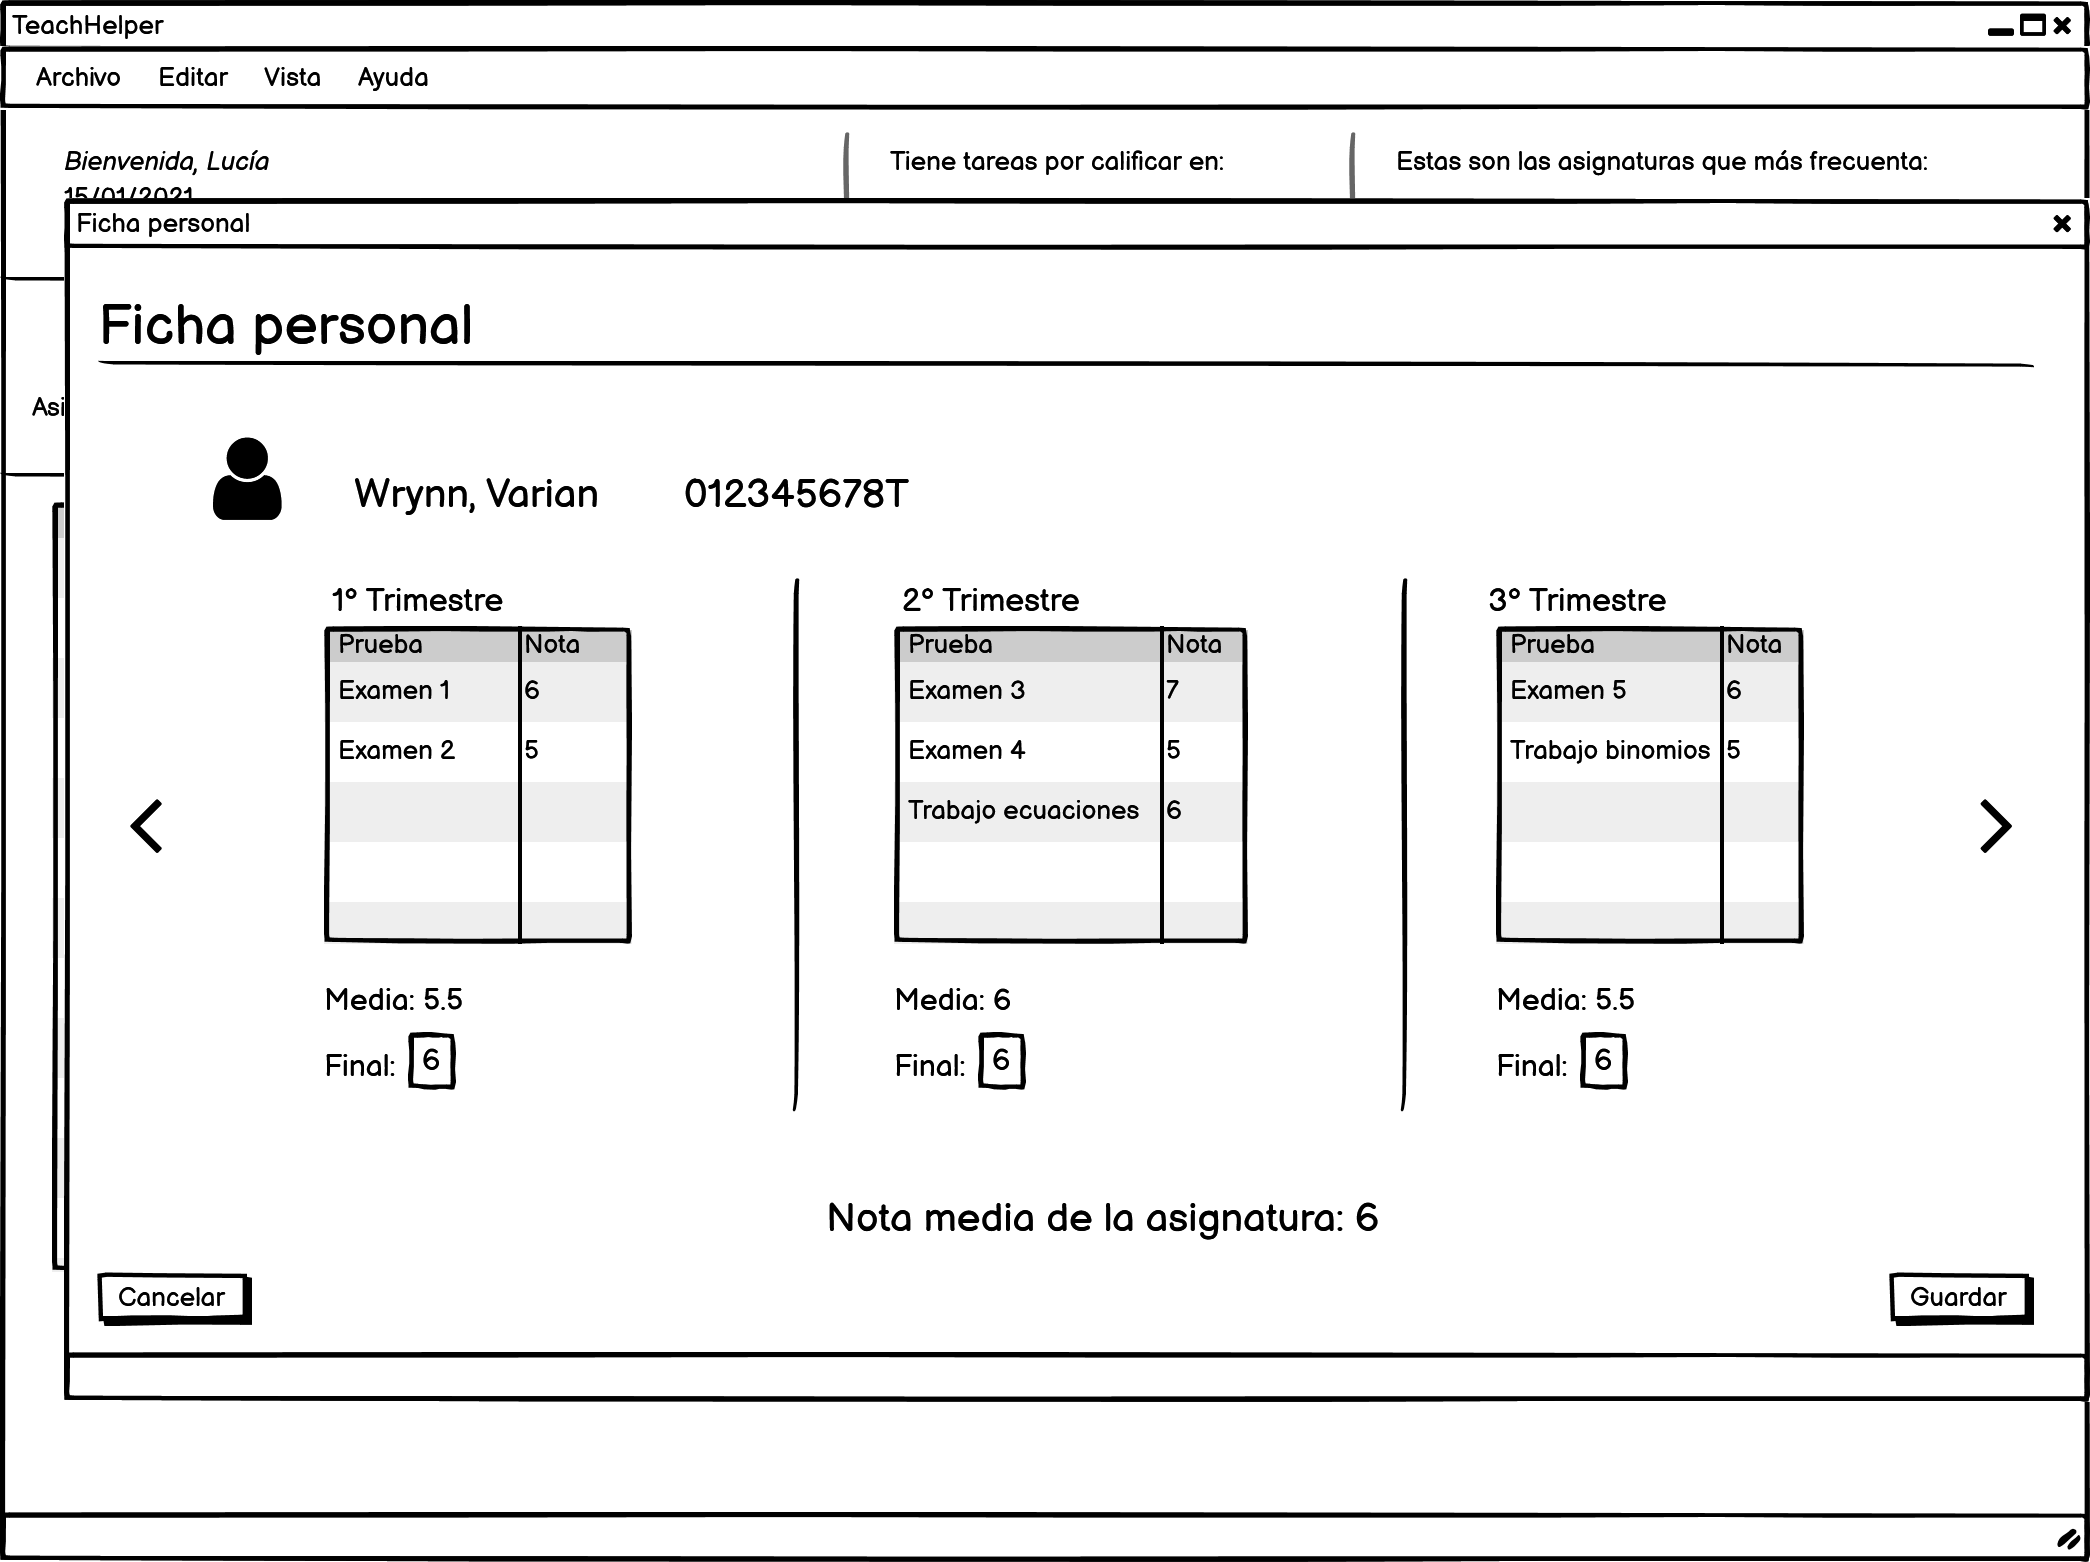
\includegraphics[width=1\linewidth]{figs/mockup_informealumno.png}
\caption{Prototipo del informe del alumnado.}
\label{Fig:mockup_informealumno}
\end{figure}

\newpage

\section{Histórico de la estructura de la base de datos}
\label{ana:db}
En esta sección se muestran todos los cambios que ha sufrido la estructura de la base de datos durante el desarrollo de la aplicación.

La figura \ref{Fig:ADB_Definition_1} muestra una primera definición de la base de datos, con 9 tablas, de las que solo 2 de ellas serían tablas ''muchos a muchos'' y no corresponderían con un objeto en Java.

\begin{figure}[H]
\centering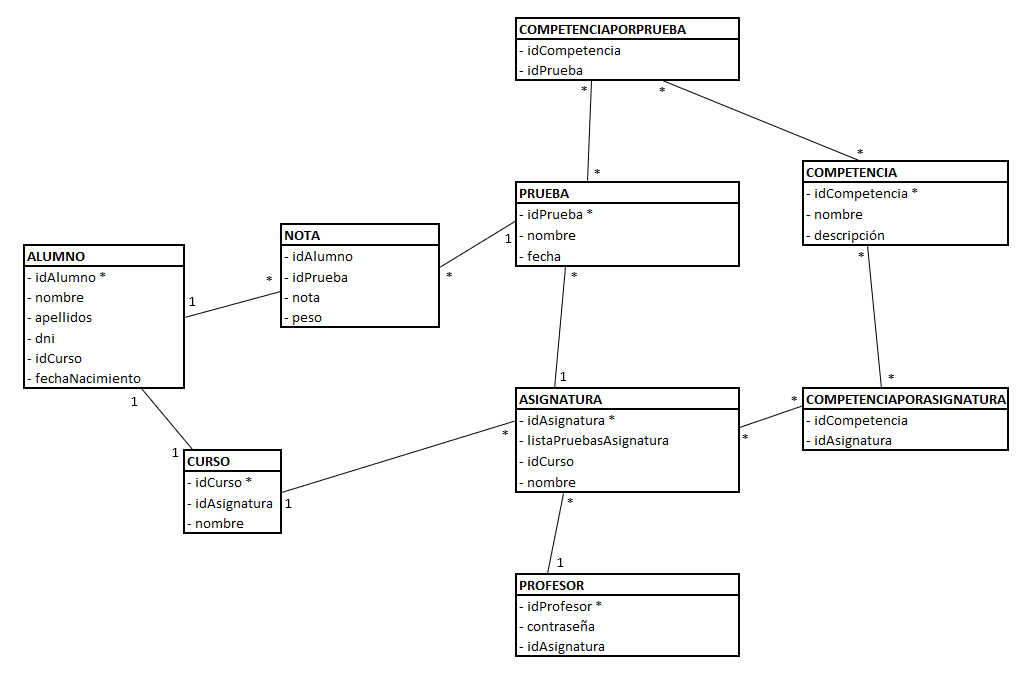
\includegraphics[width=1\linewidth]{figs/DB_Definition_1.png}
\caption{Definición primitiva de la base de datos.}
\label{Fig:ADB_Definition_1}
\end{figure}

\newpage
La segunda definición de la base de datos, en la figura \ref{Fig:ADB_Definition_2}, muestra cómo la tabla PROFESOR, que contenía los datos de un docente, se dividió en DATOSSESION y MAESTRO, para almacenar por separado los datos de inicio de sesión del docente y las asignaturas que imparta.

Además se crea la tabla ASIGNATURASENCURSO, para almacenar las asignaturas pertenecientes a un curso y evitar así la multiplicidad innecesaria en la tabla CURSO de la definición anterior.

\begin{figure}[H]
\centering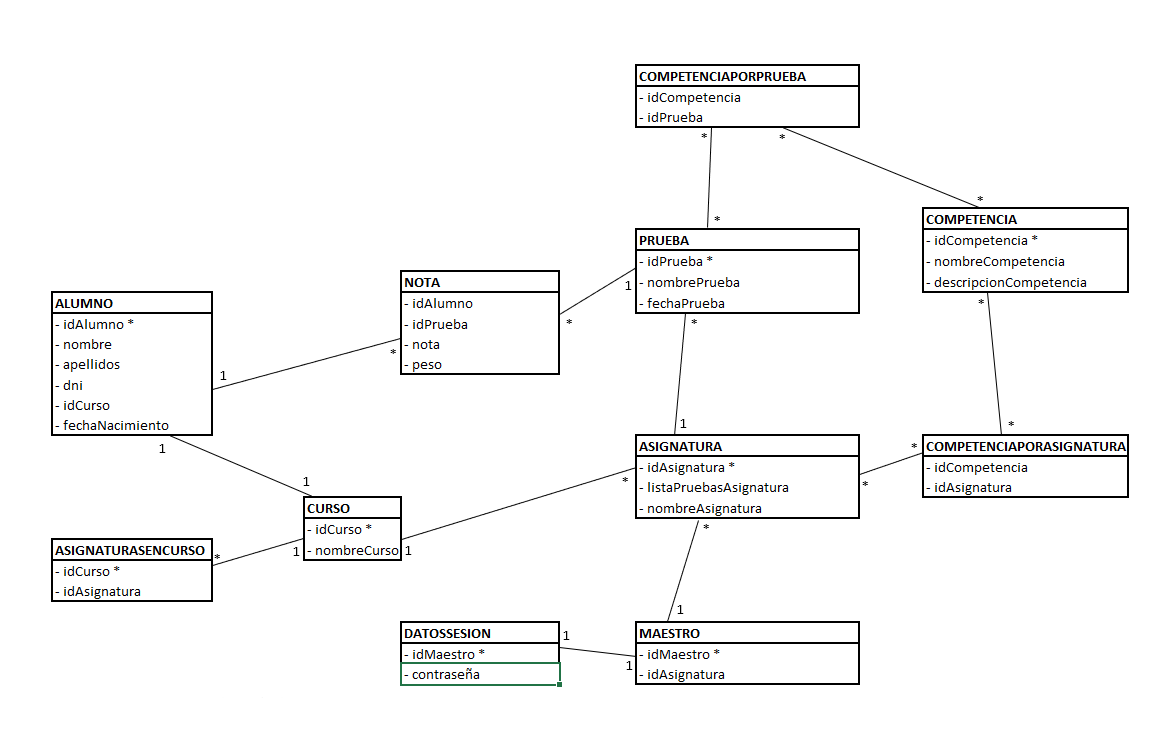
\includegraphics[width=1\linewidth]{figs/DB_Definition_2.png}
\caption{Segunda definición de la estructura de la base de datos.}
\label{Fig:ADB_Definition_2}
\end{figure}

\newpage
En la figura \ref{Fig:ADB_Definition_3} podemos ver la tercera iteración en el proceso de modelado de la base de datos. En este momento se notó que en la tabla NOTA no se podrían almacenar las notas finales del alumno, dado que de estas hay una por trimestre, y en esta tabla no se tiene en cuenta ese aspecto. Para ello, se creó la tabla NOTAFINAL.

\begin{figure}[H]
\centering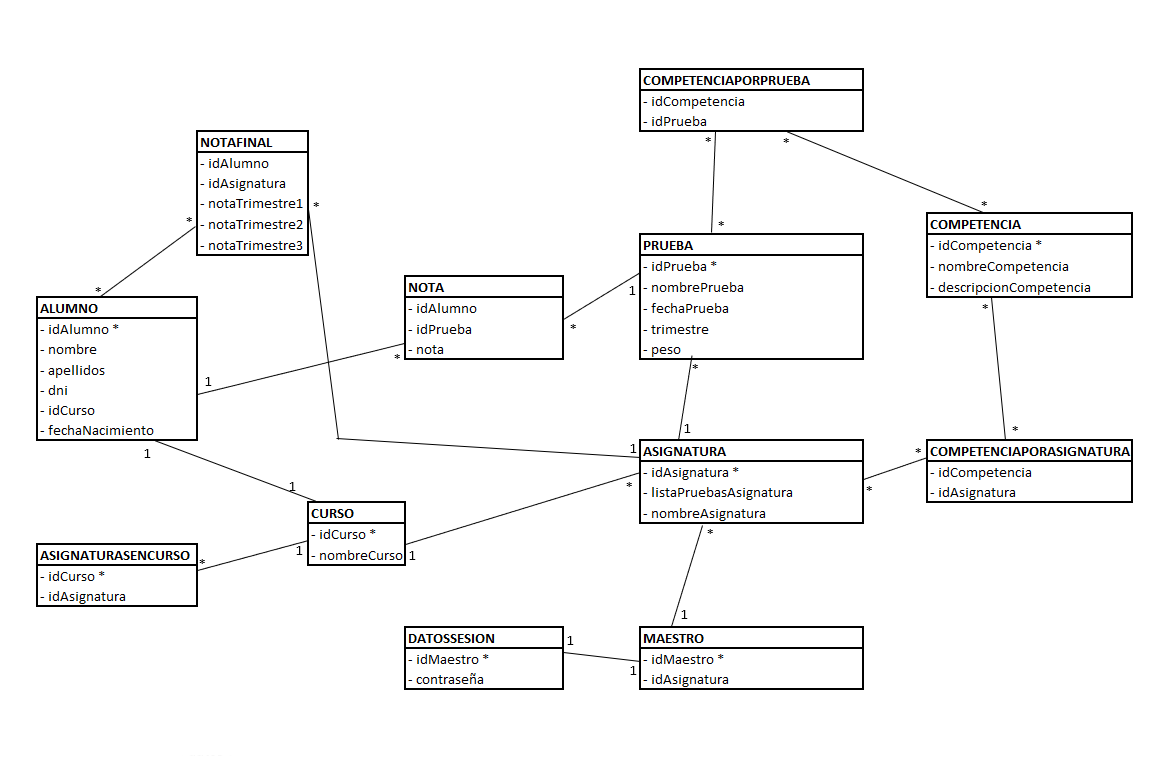
\includegraphics[width=1\linewidth]{figs/DB_Definition_3.png}
\caption{Tercera definición de la estructura de la base de datos.}
\label{Fig:ADB_Definition_3}
\end{figure}

\newpage
La figura \ref{Fig:ADB_Definition_4} muestra la cuarta definición de la estructura de la base de datos, que sufrió un cambio para permitir diferenciar las asignaturas troncales de las optativas. Para ello se creó la tabla ALUMNOSPOROPTATIVAS, que almacenaría los alumnos que estuvieran en cada una de las asignaturas optativas.

\begin{figure}[H]
\centering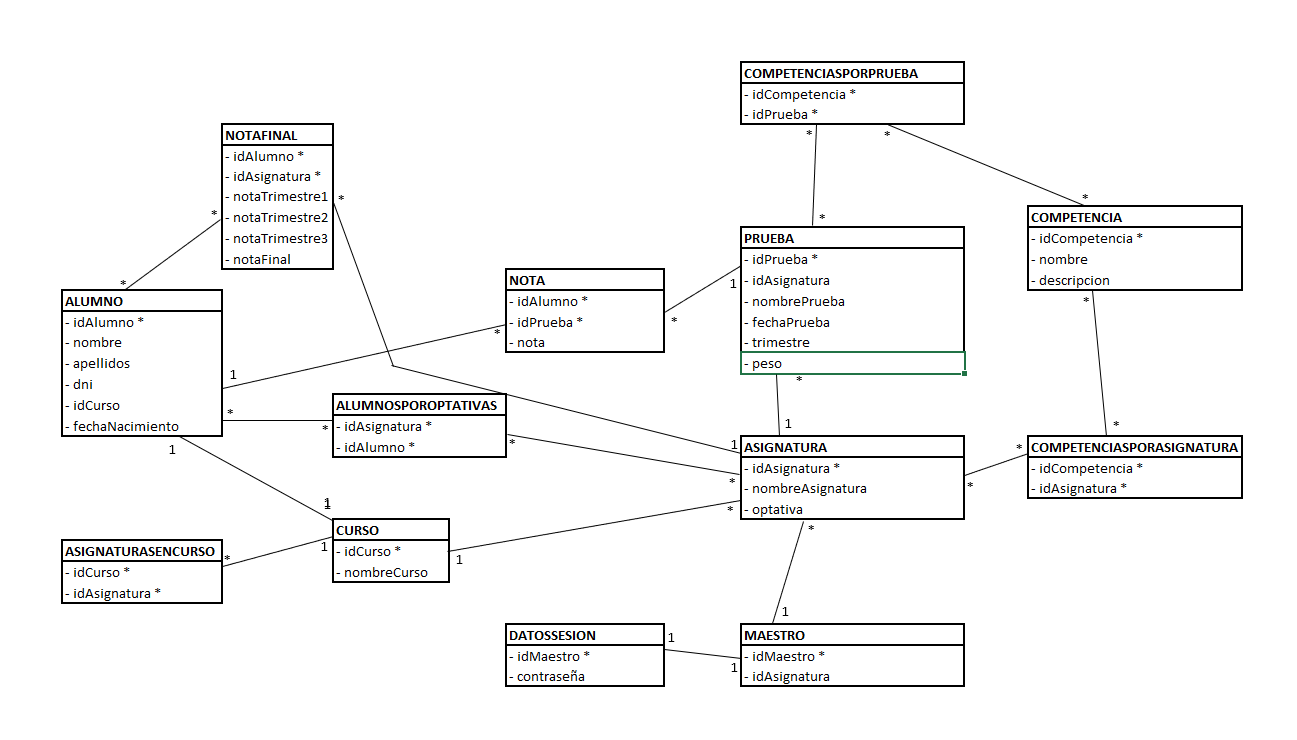
\includegraphics[width=1\linewidth]{figs/DB_Definition_4.png}
\caption{Cuarta definición de la estructura de la base de datos.}
\label{Fig:ADB_Definition_4}
\end{figure}

\newpage
El caso de las asignaturas optativas, que no se tuvo en cuenta desde un inicio, fue un problema mayor. En la figura \ref{Fig:ADB_Definition_5} se puede volver a notar un cambio referente a este tema: los alumnos debían ser clasificados por asignaturas en vez de por cursos, ya que el diseño con la tabla ALUMNOSPOROPTATIVAS no tenía cohesión con el resto de la definición, al no haber una tabla ALUMNOSPORTRONCALES. Esto se arregló relacionando los alumnos directamente con las asignaturas mediante una tabla ALUMNOSPORASIGNATURA, donde se almacenarían los dos tipos de asignatura, y los alumnos que pertenecieran a ellas. De esta forma, para diferenciar si una asignatura era optativa o troncal, se usaba el campo ''optativa'' en la tabla ASIGNATURA.

\begin{figure}[H]
\centering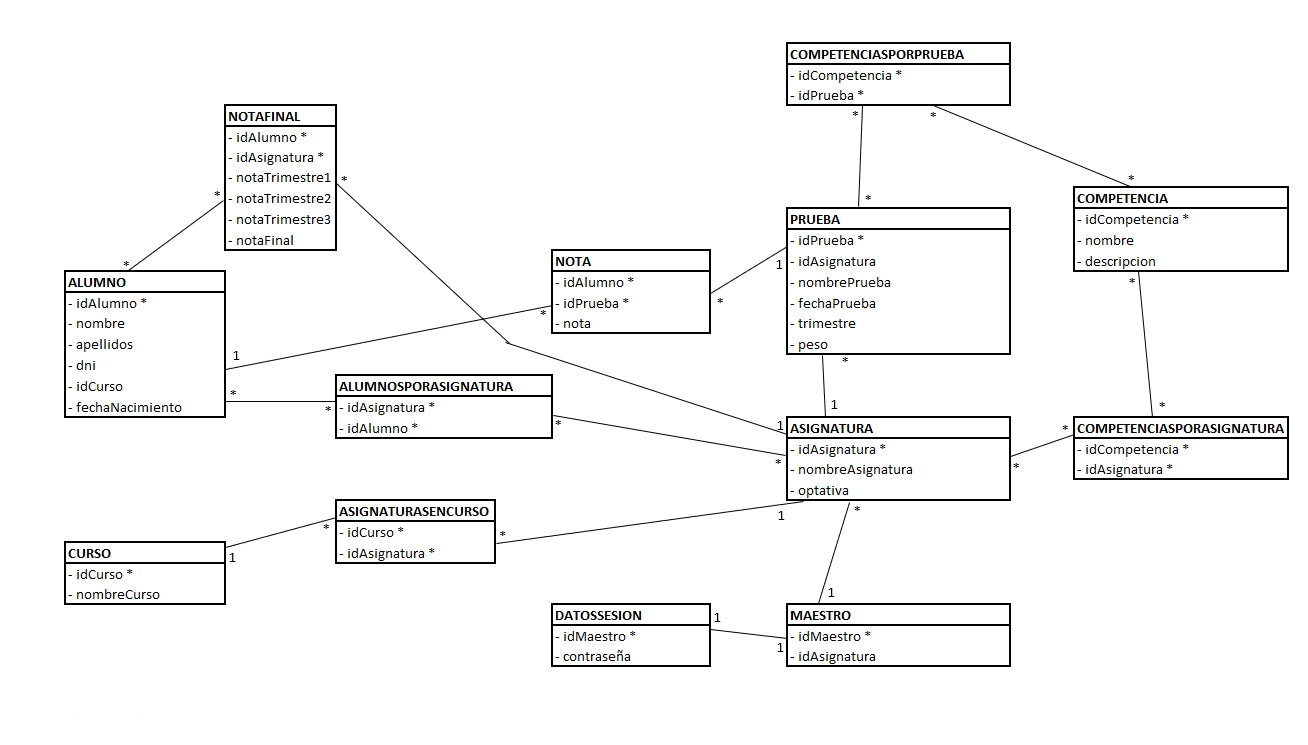
\includegraphics[width=1\linewidth]{figs/DB_Definition_5.png}
\caption{Quinta definición de la estructura de la base de datos.}
\label{Fig:ADB_Definition_5}
\end{figure}

\newpage
Finalmente, en la figura \ref{Fig:ADB_Definition_6} se pueden apreciar dos pequeños cambios, con los que finalizaron las iteraciones para encontrar la estructura definitiva de la base de datos. Estos cambios son: supresión del idAsignatura en la tabla ASIGNATURA, ya que esta información estaba duplicada en la tabla ALUMNOSPORASIGNATURA. Además, se decidió crear un título más pequeño para las pruebas, al que se llamó etiqueta, en la tabla PRUEBA.

\begin{figure}[H]
\centering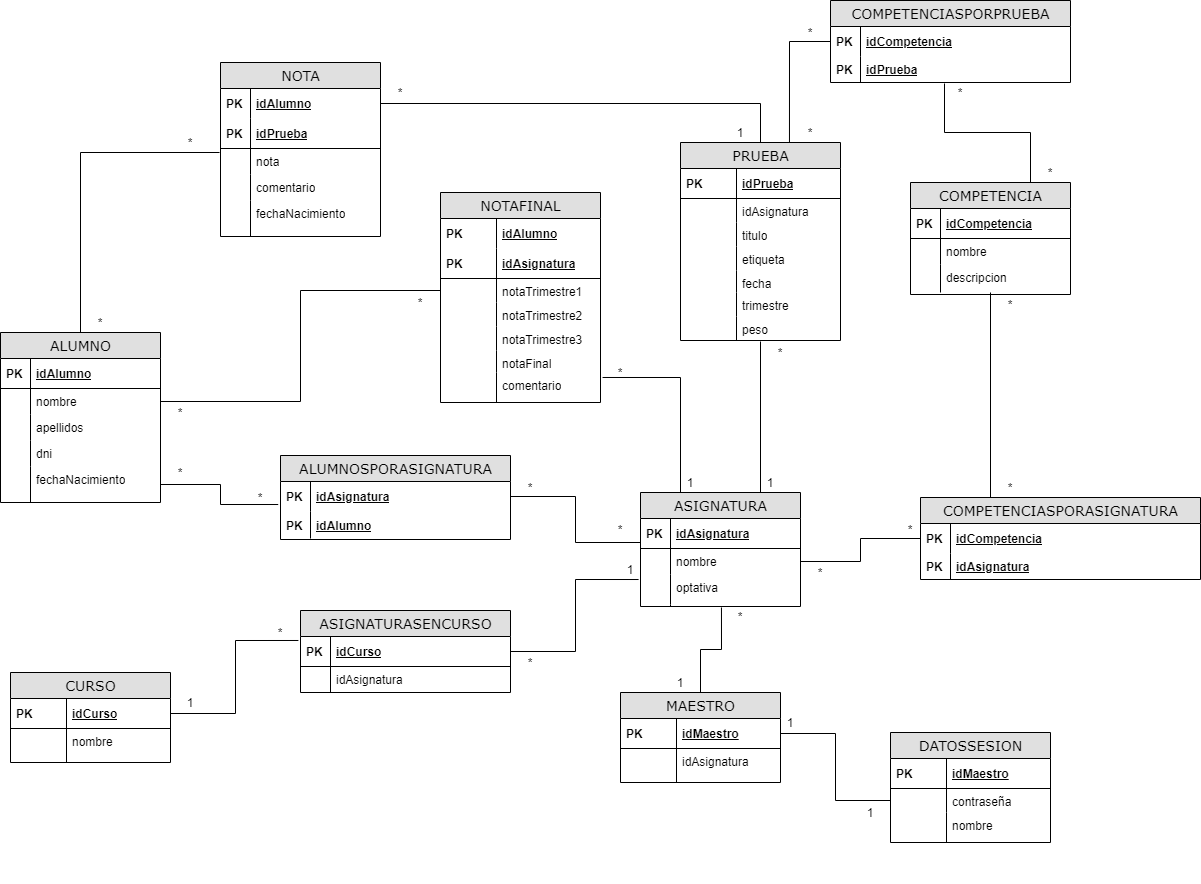
\includegraphics[width=1\linewidth]{figs/DB_Definition_6.png}
\caption{Estructura definitiva de la base de datos.}
\label{Fig:ADB_Definition_6}
\end{figure}

\newpage

\section{Diagrama de clases}
\label{ana:clases}
En esta sección se muestra el diagrama de clases correspondiente a la aplicación.

\begin{sidewaysfigure}[]
  \centering
  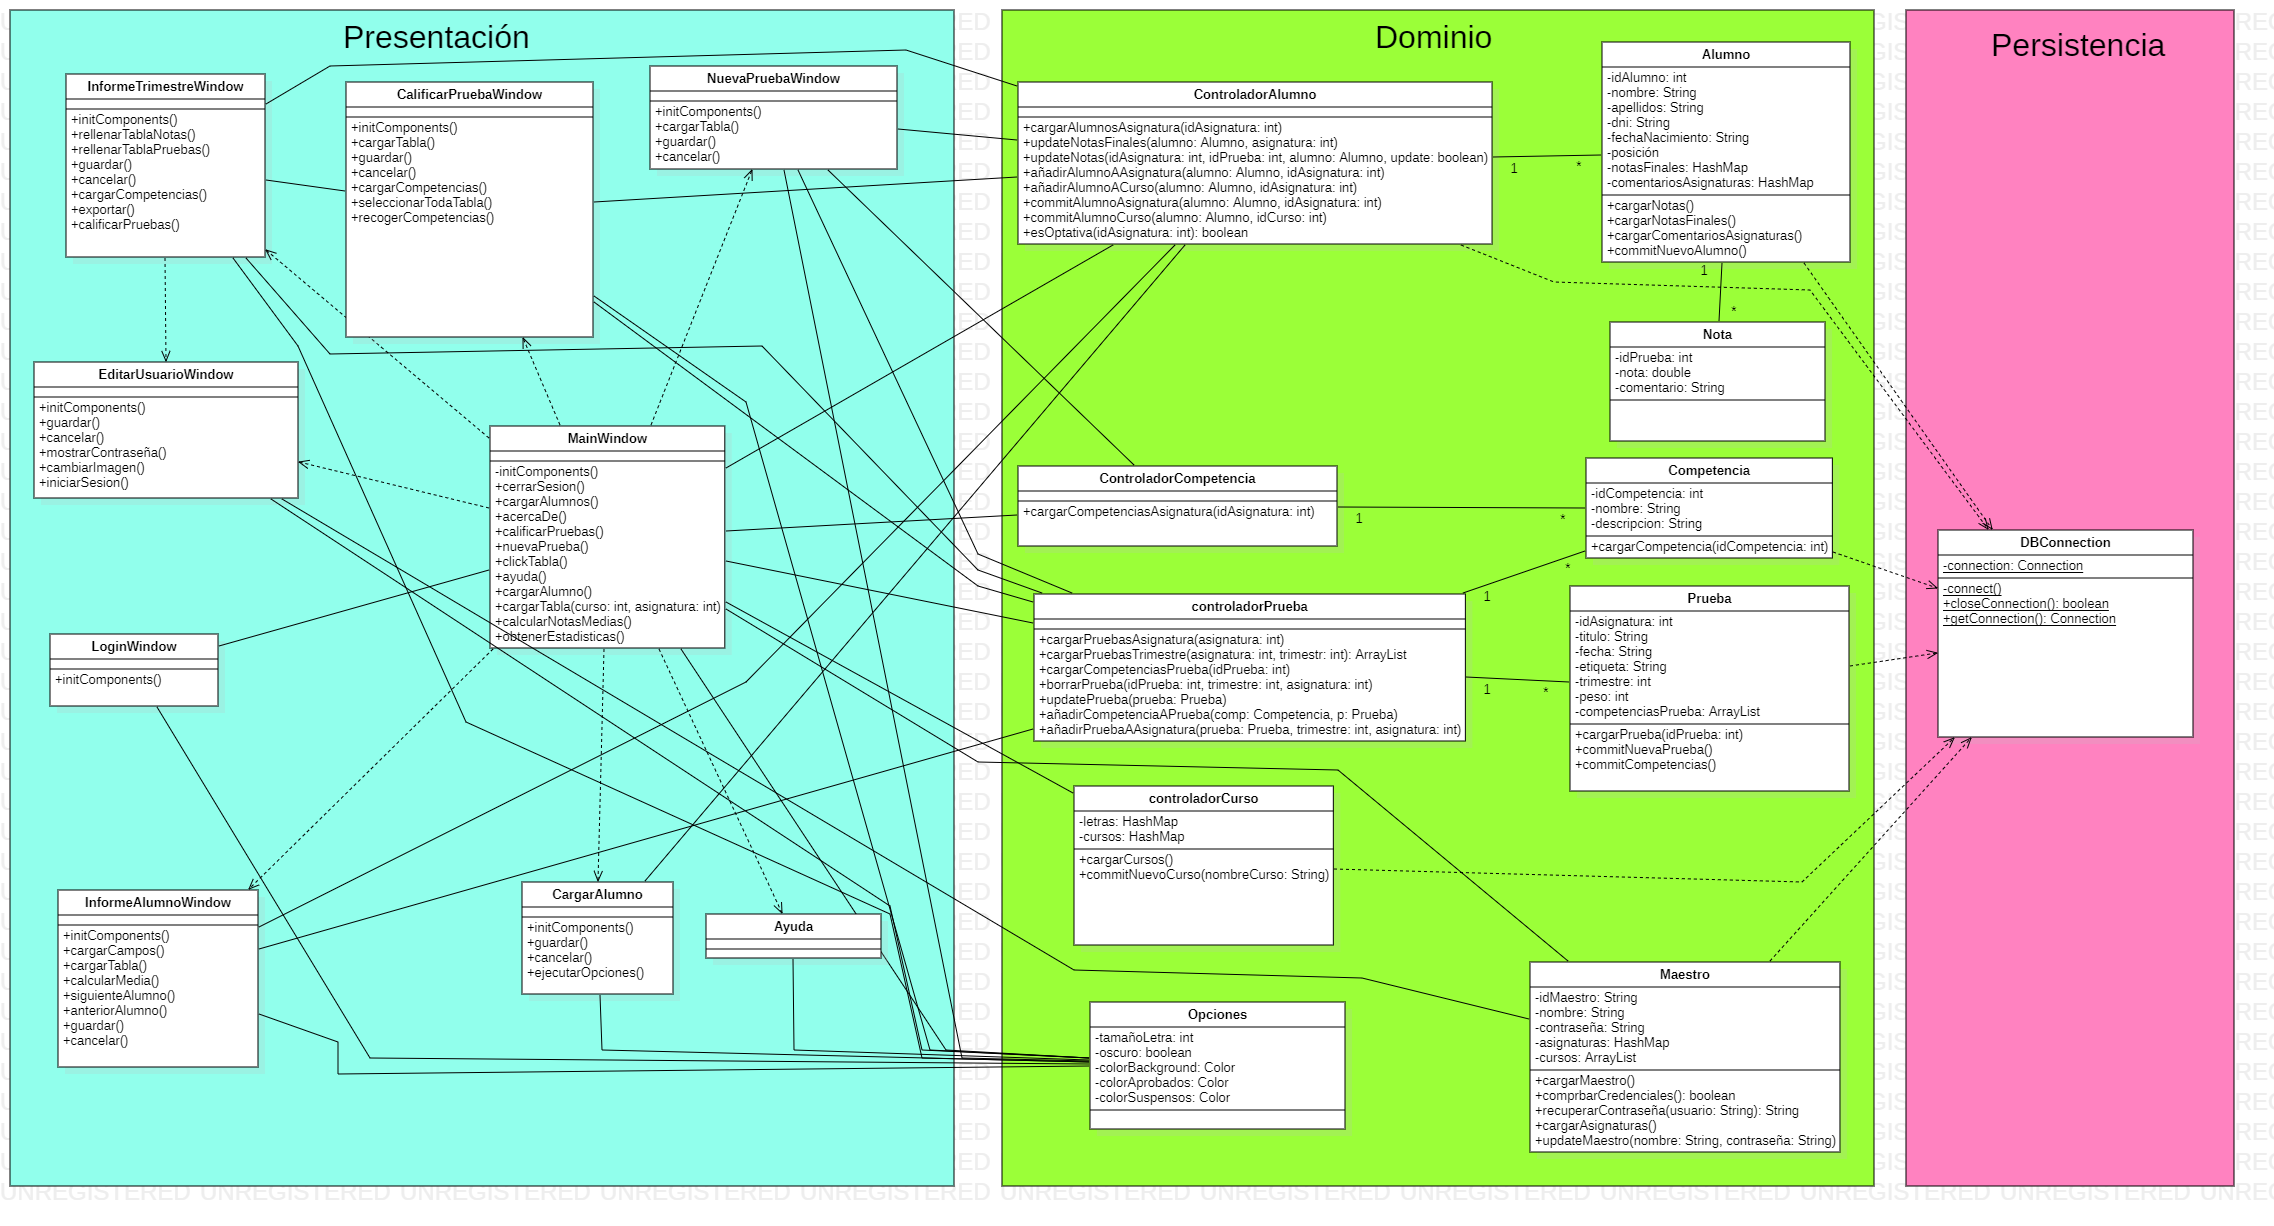
\includegraphics[width=1\linewidth]{figs/ClassDiagram.png}
\end{sidewaysfigure}

\begin{figure}[H]
\centering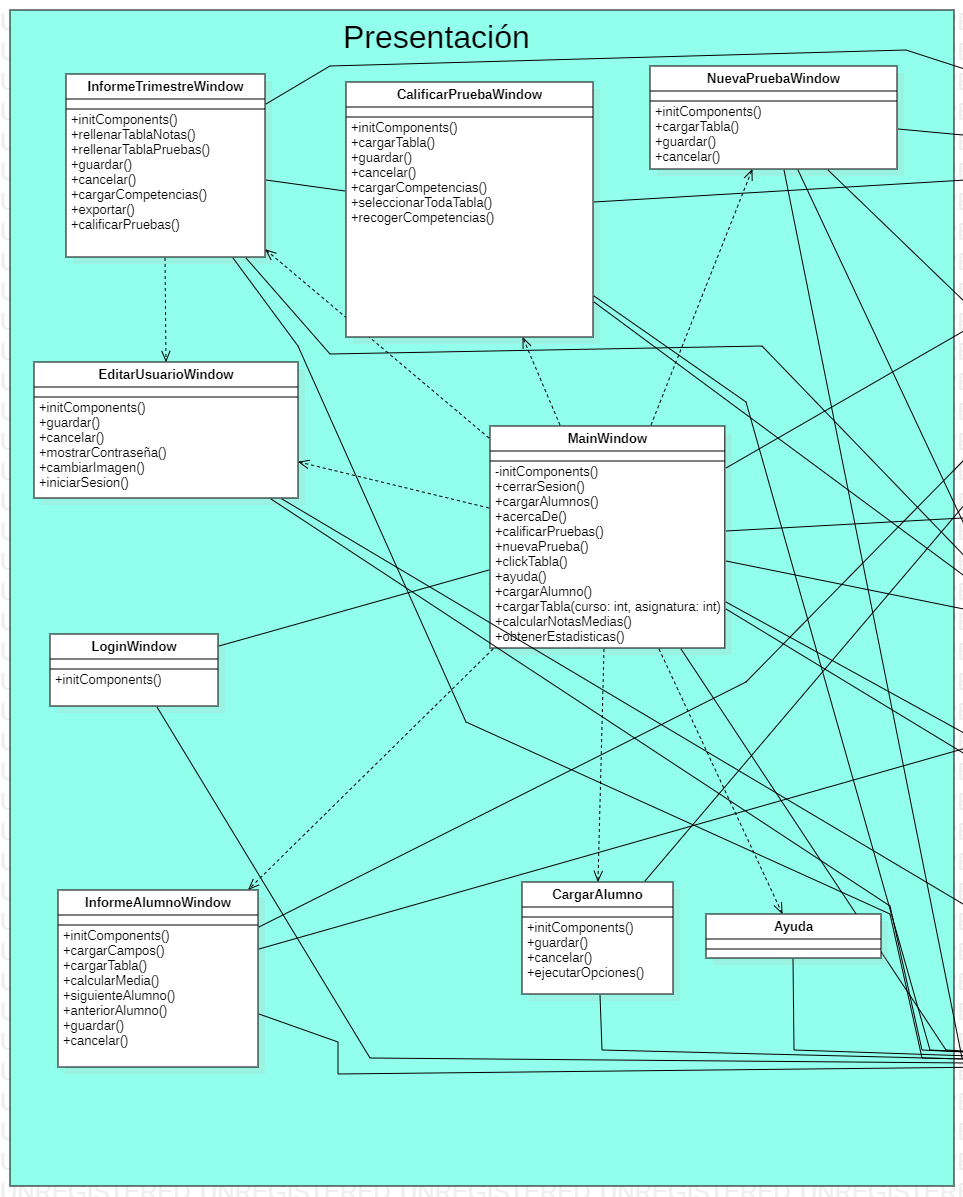
\includegraphics[width=1\linewidth]{figs/ClassDiagramPres.png}
\end{figure}

\begin{figure}[H]
\centering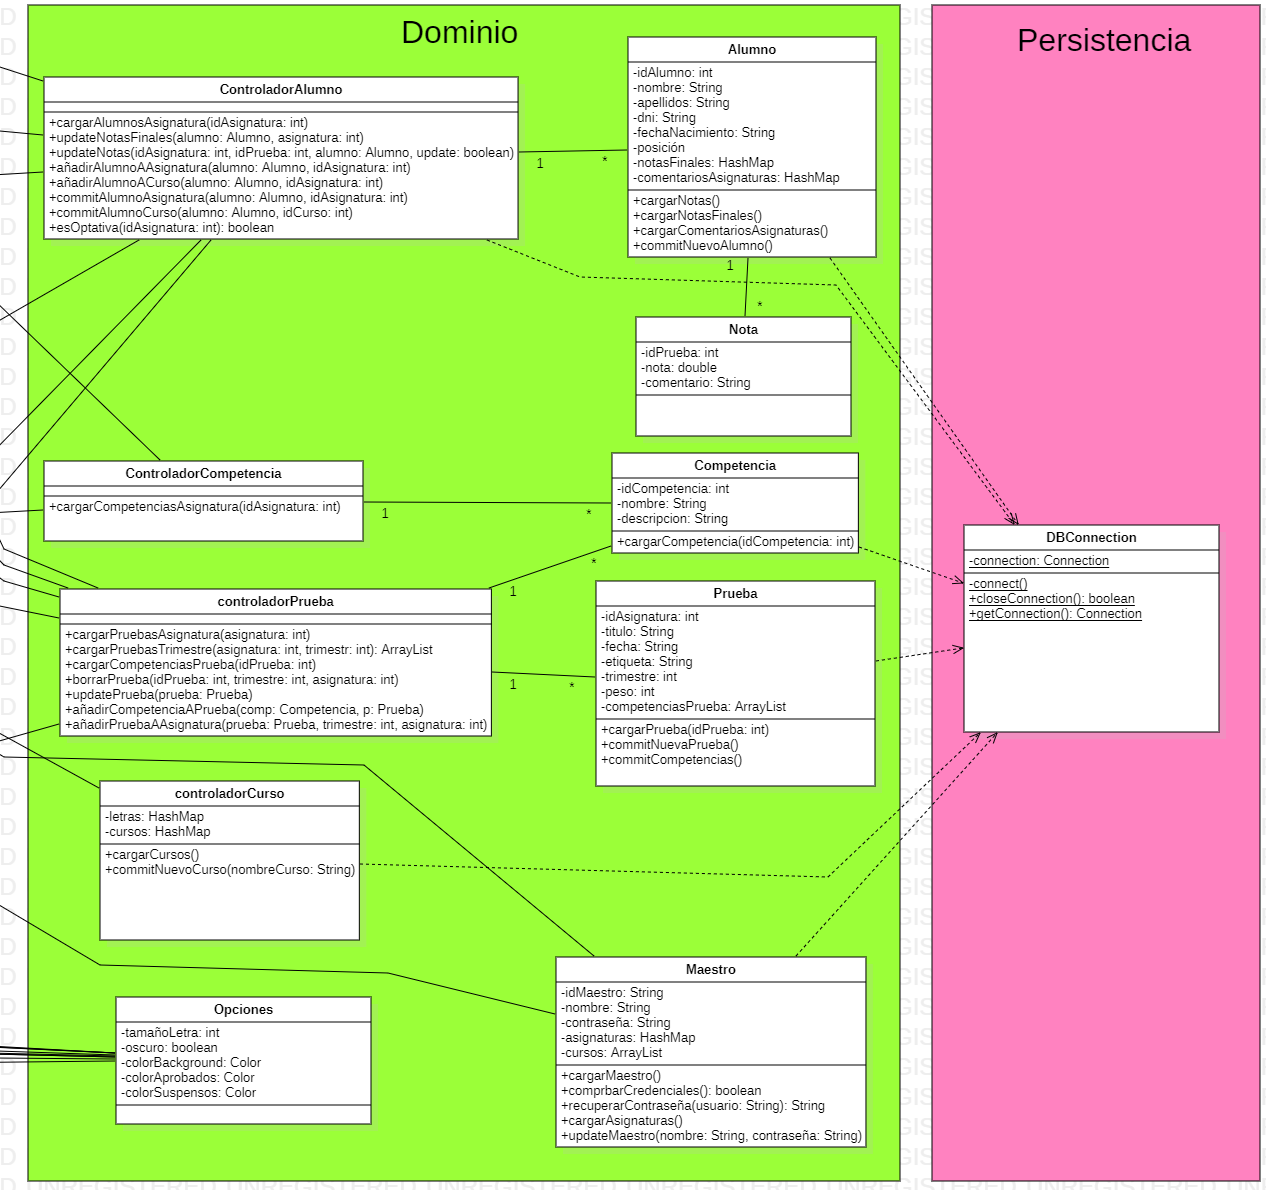
\includegraphics[width=1\linewidth]{figs/ClassDiagramDom.png}
\end{figure}